\documentclass[article]{jss}

%% sealedge JSS manuscript (camera-ready draft; plain LaTeX, not .Rnw)
%% Compile: pdflatex + bibtex + pdflatex x2
%% Numbers in case-study tables MUST match replication/output_paper_grade/results.json

\usepackage{orcidlink,thumbpdf,lmodern}
\usepackage{booktabs}
\usepackage{tabularx}
\usepackage{tikz}
\usetikzlibrary{arrows.meta,positioning,fit,calc}

\newcommand{\class}[1]{`\code{#1}'}
\newcommand{\fct}[1]{\code{#1()}}

%% Break long monospace identifiers/paths in justified text.
%% Inside \code, \_ becomes underscore + break opportunity.
\makeatletter
\DeclareRobustCommand{\code}[1]{%
  \bgroup\ttfamily
  \def\_{\char`\_\allowbreak}%
  #1%
  \egroup
}
\makeatother
\emergencystretch=3em
\tolerance=2000

%% -- metainformation ---------------------------------------------------------
\author{
  Hansen Winarto\\
  Bina Nusantara University
}
\Plainauthor{Hansen Winarto}

\title{\pkg{sealedge}: Sealed Holdouts and Multiple-Testing Defaults for Crypto Backtests in \proglang{Python}}
\Plaintitle{sealedge: Sealed Holdouts and Multiple-Testing Defaults for Crypto Backtests in Python}
\Shorttitle{\pkg{sealedge}: Sealed Holdouts for Crypto Backtests}

\Abstract{
  \pkg{sealedge} is a \proglang{Python} package that implements sealed-holdout
  evaluation and multiple-testing defaults for strategy backtests, with a
  focus on cryptocurrency perpetual markets as the application domain.
  The package ships HMAC-SHA256 sealing of holdout inputs
  \citep{Krawczyk+etal:1997}, an explore/commit application programming
  interface (API) in which exploration never opens the seal, Probabilistic
  Sharpe Ratio (PSR) and deflated-Sharpe diagnostics
  \citep{Bailey+LopezDePrado:2012,Bailey+LopezDePrado:2014}, Superior
  Predictive Ability (SPA) testing with dual null constructions
  \citep{Hansen:2005,White:2000}, deterministic walk-forward analysis (WFA)
  \citep{Pardo:2008}, and supporting multiplicity tools including
  Benjamini--Hochberg false discovery rate (FDR) control
  \citep{Benjamini+Hochberg:1995}.  The public distribution name is
  \pkg{sealedge}; the importable package remains \pkg{quant\_lib}.  Three registered
  perpetual-futures experiments illustrate the public explore path.  Paper-grade SPA
  $p$-values come from a single replication run with \code{n\_spa\_iters = 2000} and
  include both rejections and non-rejections.
}

\Keywords{backtesting, cryptocurrency, multiple testing, Probabilistic Sharpe Ratio, Superior Predictive Ability, walk-forward analysis, \proglang{Python}, reproducible research}
\Plainkeywords{backtesting, cryptocurrency, multiple testing, Probabilistic Sharpe Ratio, Superior Predictive Ability, walk-forward analysis, Python, reproducible research}

\Address{
  Hansen Winarto\\
  Information Systems Department, BINUS Online Learning,\\
  Bina Nusantara University,\\
  Jakarta, Indonesia 11480\\
  E-mail: \email{hansenwinarto@binus.ac.id}\\
  URL: \url{https://github.com/Hansiongs/sealedge}
}

\begin{document}

%% -- 1 Introduction ----------------------------------------------------------
\section[Introduction]{Introduction} \label{sec:intro}

\pkg{sealedge} is a \proglang{Python} package for sealed-holdout strategy
evaluation and multiple-testing defaults
\citep{sealedge,Python}.  It packages established statistical and research-design
tools: HMAC-authenticated holdout seals \citep{Krawczyk+etal:1997},
Probabilistic and deflated Sharpe diagnostics
\citep{Bailey+LopezDePrado:2012,Bailey+LopezDePrado:2014}, Superior Predictive
Ability (SPA) and reality-check testing \citep{Hansen:2005,White:2000},
walk-forward analysis \citep{Pardo:2008}, and supporting multiplicity utilities
including Benjamini--Hochberg FDR control
\citep{Benjamini+Hochberg:1995}; together these
  tools form
a single importable stack with a public explore/commit API.  The distribution
name is \pkg{sealedge}; the importable package remains \pkg{quant\_lib} for API
stability (Section~\ref{sec:architecture}).  No new Sharpe estimator, SPA
theorem, or FDR procedure is proposed.  The software contribution is how these
methods are wired into defaults, return objects, audit surfaces, and a
replication path that does not open the holdout during exploration.

Open backtesting systems such as Backtrader, Zipline / Zipline-Reloaded,
vectorbt, and QuantConnect Lean provide strong execution and research engines
\citep{Backtrader,Zipline,vectorbt,Lean}.  Research-discipline controls
(sealed holdouts, SPA/PSR on the same objects as trades, experiment-level
multiplicity bookkeeping) are often left to the user rather than shipped as
package defaults (Section~\ref{sec:comparison}).  \pkg{sealedge} targets this gap by making the disciplined path the default
API surface, rather than an optional notebook appendix.

Cryptocurrency perpetual futures are the motivating application domain for the
registered experiments shipped with the package.  Continuous trading, funding
cash-flows, gaps, and abrupt volatility regimes make holdout leakage and
multiple testing easy to understate in ad-hoc scripts.  The domain motivates
defaults and illustrations; it is not a claim that the methods apply only to
crypto markets.

\subsection{Scope relative to methods and related software}

Holdout evaluation, WFA \citep{Pardo:2008}, PSR and deflated-Sharpe methods
\citep{Bailey+LopezDePrado:2012,Bailey+LopezDePrado:2014}, SPA / reality-check
testing \citep{Hansen:2005,White:2000}, stationary bootstrap constructions
used inside SPA nulls \citep{Politis+Romano:1994}, finite-sample permutation
$p$-value hygiene \citep{Phipson+Smyth:2010}, and FDR control
\citep{Benjamini+Hochberg:1995} are established.  \pkg{sealedge} implements
them on engine return objects and research-session state: sealed holdout
inputs, explore that never breaks the seal, commit as an explicit second step,
SPA/PSR reporting, deterministic WFA with recorded trials (including
\pkg{Optuna}-based search \citep{Akiba+etal:2019} and a \pkg{Numba} bar engine
\citep{Lam+etal:2015}), and journal-level multiplicity context for Bonferroni
and FDR bookkeeping.  Section~\ref{sec:background} reviews the methods;
Section~\ref{sec:capabilities} maps primary claims and additional statistical
tools to modules and APIs.

\subsection{Contributions}

Concrete surfaces shipped by the package:

\begin{enumerate}
  \item An HMAC-SHA256 sealed-holdout workflow in which explore never opens
    the seal and commit re-verifies then breaks it once
    (Section~\ref{sec:capabilities}).
  \item Integrated PSR and deflated-Sharpe diagnostics on the same trade and
    return objects produced by the engine, including weighted effective sample
    size constructions \citep{Kish:1965}.
  \item SPA testing with dual-null software options, Phipson--Smyth $p$-value
    formation, and paper-grade defaults (\code{n\_spa\_iters = 2000} in the
    canonical replication path).
  \item Deterministic, seedable walk-forward analysis as an engineered
    realization of established WFA practice, with recorded trials and purge
    policy.
  \item Supporting multiplicity and process tools, including Benjamini--Hochberg
    FDR, journal Bonferroni context, bootstrap helpers, hypothesis
    pre-registration fields, and a public \code{tools.stats} facade, shipped
    beside the four primary claims (Section~\ref{sec:capabilities}).
  \item An empirical illustration on three registered perpetual-futures
    experiments that exercises the public explore path and reports mixed SPA
    outcomes from the paper-grade replication sample
    (Section~\ref{sec:cases}, Table~\ref{tab:spa}):
    \code{vol\_compression\_v1}, \code{pullback\_sniper\_rsi}, and
    \code{funding\_rate\_carry}.
\end{enumerate}

%% -- 2 Background ------------------------------------------------------------
\section[Background]{Background} \label{sec:background}

Background material below is limited to methods the package implements;
packaging into defaults, APIs, and audit surfaces is deferred to
Section~\ref{sec:capabilities}.

\subsection{Holdout evaluation and the peeking problem}

A standard way to limit overfit is to reserve a terminal holdout window,
fit or select on earlier data only, and evaluate the holdout once.
In trading research the same idea appears as an out-of-sample block after
an in-sample optimization period.  The difficulty is operational rather than
conceptual: analysts can still look at the reserved window while
tuning, silently extend features that depend on post-sample information, or
re-run selection until the holdout ``works.''

Cryptographic sealing does not invent a new validation design.  It applies
standard hash-and-authenticate primitives (here HMAC-SHA256 over holdout
OHLCV and related warmup ranges) so that any modification of sealed inputs
is detectable and so that the default exploratory path never opens the
reserved window.  The methodological content remains ordinary holdout
evaluation; the enforcement problem is what the software targets.

\subsection{Probabilistic Sharpe Ratio and selection-aware performance}

The Sharpe ratio remains a common scalar summary of a return path, but it
is sensitive to non-normality and to selection across many trials.
\citet{Bailey+LopezDePrado:2012,Bailey+LopezDePrado:2014} discuss Probabilistic Sharpe Ratio (PSR)
and deflated-Sharpe style corrections that account for estimation error,
skewness and kurtosis, and the inflation that arises when the reported
strategy is the winner of a search.  Related practice also tracks effective
sample size under dependence and applies multiple-comparison adjustments
when many symbols or trials are scored together.

\pkg{sealedge} treats these diagnostics as implementations to ship,
not as notebook formulas reviewers must re-derive.  Background for the
paper is therefore the published PSR / deflated-Sharpe literature, not a
new performance theory.

\subsection{Data snooping, reality check, and SPA}

When many forecasts or trading rules are compared on the same history,
conventional $t$-tests on the winner are anti-conservative.
\citet{White:2000} formalizes a reality-check perspective on data snooping;
\citet{Hansen:2005} develops the Superior Predictive Ability (SPA) test,
including recentering and studentization choices that improve behavior
relative to naive benchmarks when many poor alternatives are present.

Finite-sample Monte Carlo or permutation $p$-values raise a further
practical issue: a raw count of extremes can produce a reported $p$-value
of exactly zero.  \citet{Phipson+Smyth:2010} show why permutation $p$-values
should not be zero when permutations are randomly drawn and recommend
add-one style corrections.  \pkg{sealedge} uses that finite-sample hygiene
in its SPA reporting paths.

Across many registered experiments or many simultaneous $p$-values, the package
also ships Benjamini--Hochberg FDR correction \citep{Benjamini+Hochberg:1995}
and journal-level Bonferroni context; these multiplicity tools are secondary to
the four primary claims and are detailed with the additional statistical
surfaces in Section~\ref{sec:capabilities}.

Two points matter for reading the empirical illustration.  First, SPA answers a
specific null about superior predictive ability under a chosen resampling
construction; it is not a substitute for economic interpretation of costs,
turnover, or capacity.  Second, non-rejection under the configured null is a
possible SPA result.  The paper-grade sample therefore reports both rejections
and non-rejections without treating either as a software defect.

\subsection{Walk-forward analysis}

Walk-forward analysis (WFA) optimizes a strategy on a rolling or anchored
in-sample window, evaluates the next out-of-sample segment, then advances
the window \citep{Pardo:2008}.  Purge or embargo gaps are commonly inserted
so that features with long lookbacks do not leak across the in-sample /
out-of-sample boundary.  WFA is a research protocol, not a single
closed-form estimator: implementations differ in optimizer, objective,
parameter freezing rules, and how multi-asset portfolios rebalance risk
across folds.

Here WFA is background practice that the package realizes
deterministically (fixed seeds, recorded trials, adaptive purge policy).
Claims about novelty attach to the engineering of that realization and to
its integration with sealed holdout and SPA/PSR reporting
(Sections~\ref{sec:design}--\ref{sec:capabilities}), not to inventing
walk-forward testing as a statistical method.

%% -- 3 Design principles -----------------------------------------------------
\section[Design principles]{Design principles} \label{sec:design}

The package is organized around a small set of product rules enforced by the
public API and session state machine, not optional style advice for notebook
users.

When a \code{ResearchSession} is constructed, holdout-range inputs are hashed
and bound under HMAC-SHA256 (Section~\ref{subsec:claim-seal}).  Opening the
holdout is not a configuration flag on explore; it is a subsequent
\fct{run\_commit} operation that re-verifies the seal and records a one-shot
break.

\fct{run\_explore} and the default replication script never break the seal and
never return holdout PSR.  \fct{run\_commit} requires stage \code{ready},
re-verifies hashes against cached payloads, opens the holdout once, and only
then scores commit-path diagnostics.  Reviewers can re-run explore without
consuming the holdout.

Walk-forward optimization uses a fixed global seed, per-fold seed algebra, and
recorded trial configuration so that a named experiment plus seed reconstructs
the same search path (Section~\ref{subsec:claim-wfa}).  Purge gaps and
per-symbol Optuna searches are part of that engineered path, not ad-hoc
notebook state.

\paragraph{Costs and rejections are exposed.}
Execution metrics report executed versus rejected trades and costed equity
paths.  A large signal fire-rate is visible in trade counts and rejections, not
hidden behind a single Sharpe number.  SPA and PSR consume those costed
objects, so friction is inside the statistic rather than a post-hoc footnote.

The canonical replication path fixes \code{n\_spa\_iters = 2000} and does not
ship a reduced-iteration manuscript script.  The paper-grade sample retains
whatever SPA outcomes the registered experiments produce under that budget,
including non-rejection.

Strategies enter the system as registered hypothesis objects (mechanism,
boundaries, success language, period, universe).  The candidate state machine
\[
  \texttt{hypothesis}
  \rightarrow
  \texttt{universe}
  \rightarrow
  \texttt{edge}
  \rightarrow
  \texttt{narrowed}
  \rightarrow
  \texttt{ready}
\]
blocks invalid backward transitions and stage skips so the state machine blocks exploratory mutation of a frozen claim.  Commit is only legal from
\code{ready}.

%% -- 4 Architecture ----------------------------------------------------------
\section[Software architecture]{Software architecture} \label{sec:architecture}

The distribution name on package indexes is \pkg{sealedge}
\citep{sealedge}.  The importable
\proglang{Python} package name remains \pkg{quant\_lib} for API stability:
\begin{Code}
import quant_lib
from quant_lib import run_explore, run_commit
\end{Code}
The command-line entry point is \code{quant\_exp}.  Manuscript text uses
\pkg{sealedge} for the product and \pkg{quant\_lib} for importable modules.

Modules form a one-way dependency stack from experiment configuration to the
Numba engine (names are package paths under \pkg{quant\_lib}):
\begin{Code}
experiments/  -> cli/  -> research/ -> audit/  -> tools/ -> core/  -> utils/
  registry     Typer    session      seal       API       engine    shared
\end{Code}
\begin{itemize}
  \item \code{experiments/}: named strategy registrations (period, universe,
    hypothesis metadata, search spaces).
  \item \code{cli/}: \code{quant\_exp} commands for list, explore, commit, and
    reporting without a custom driver script.
  \item \code{research/}: session lifecycle, explore pipeline, candidate stages,
    commit path, result objects, optional plotting.
  \item \code{audit/}: holdout seal types, hypothesis factories, experiment
    journal multiplicity bookkeeping.
  \item \code{tools/}: public research helpers, including the \code{stats}
    facade for SPA/PSR/FDR.
  \item \code{core/}: features, WFA, SPA, metrics, and the \pkg{Numba}
    \code{@njit} bar engine \citep{Lam+etal:2015} under costs and constraints.
  \item \code{utils/}: shared primitives without pulling research state.
\end{itemize}

\begin{figure}[t!]
\centering
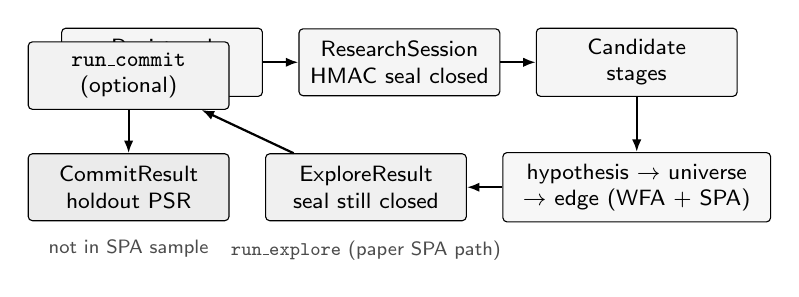
\begin{tikzpicture}[
  font=\footnotesize\sffamily,
  box/.style={draw, rounded corners=1.5pt, align=center,
    inner sep=4pt, minimum height=0.85cm, minimum width=2.55cm},
  arr/.style={-{Latex[length=1.6mm]}, thick},
  note/.style={font=\scriptsize\sffamily, text=black!70}
]
  \node[box, fill=black!4] (exp) {Registered\\experiment};
  \node[box, right=0.45cm of exp, fill=black!4] (sess) {ResearchSession\\HMAC seal closed};
  \node[box, right=0.45cm of sess, fill=black!4] (cand) {Candidate\\stages};
  \node[box, below=0.7cm of cand, fill=black!3, minimum width=3.4cm] (edge)
    {hypothesis $\to$ universe\\$\to$ edge (WFA + SPA)};
  \node[box, left=0.45cm of edge, fill=black!6] (er) {ExploreResult\\seal still closed};
  \node[box, left=0.45cm of er, fill=black!8] (cr) {CommitResult\\holdout PSR};
  \node[box, above=0.55cm of cr, fill=black!5] (rc) {\texttt{run\_commit}\\(optional)};

  \draw[arr] (exp) -- (sess);
  \draw[arr] (sess) -- (cand);
  \draw[arr] (cand) -- (edge);
  \draw[arr] (edge) -- (er);
  \draw[arr] (er) -- (rc);
  \draw[arr] (rc) -- (cr);

  \node[note, below=0.12cm of er] {\texttt{run\_explore} (paper SPA path)};
  \node[note, below=0.12cm of cr] {not in SPA sample};
\end{tikzpicture}
\caption{Public explore/commit workflow.  Paper SPA tables use
  \fct{run\_explore} only.  Claim~1 seal lifecycle is checked by the
  synthetic micro-demo (Figure~\ref{fig:seal}) and
  Section~\ref{sec:compute}, not by opening registered-experiment
  holdouts.}
\label{fig:workflow}
\end{figure}

A typical explore call constructs a \code{ResearchSession} (holdout seal
created or loaded; explore may skip holdout feature materialization), builds a
\code{Candidate} from the registered experiment, then runs stages in order:
\begin{enumerate}
  \item \code{hypothesis}: bind mechanism, boundaries, and success criteria.
  \item \code{universe}: point-in-time eligibility under age and liquidity
    filters at the configured train start.
  \item \code{edge}: per-symbol WFA, OOS trade emission, portfolio simulation,
    dual-null SPA (Section~\ref{subsec:claim-spa}).
  \item \code{narrowed} / \code{ready}: optional narrowing then explicit
    \code{mark\_ready()} before commit is allowed.
\end{enumerate}
\fct{run\_explore} stops at explore metrics with the seal closed.
\fct{run\_commit} re-enters from a ready candidate, verifies the seal, breaks
once, and scores holdout fields.  Result dicts expose commensurate keys
(\code{spa\_p\_value}, trade counts, equity) so CLI, Python, and replication
scripts share one contract.

Most reviewers and users touch three entry points: (i)~registered experiment
names such as \code{vol\_compression\_v1}; (ii)~\fct{run\_explore} /
\fct{run\_commit} from \pkg{quant\_lib}; (iii)~\code{quant\_exp} for the same
flows from a shell.  Figure~\ref{fig:workflow} summarizes the sealed path.
The replication script calls the explore surface only.
Lower layers remain importable for extension, but paper claims are stated
against the public explore/commit contract, not against private core symbols.

\subsection{Using the software and documentation}
\label{sec:usage}

A typical research session uses three layers of documentation and one
sealed workflow.  The product name is \pkg{sealedge}; imports and CLI still
use \pkg{quant\_lib} and \code{quant\_exp}.

Formatted help for the library system is provided as NumPy-style docstrings
on public modules and functions, browsable API pages under the repository
\code{docs/} tree (built with \pkg{mkdocs}; \code{mkdocs build --strict}), and the narrative methodology
write-up used by contributors.  After install, interactive help is available
via the standard \proglang{Python} help system, e.g.\
\code{help(quant\_lib.run\_explore)} and module-level
\code{help(quant\_lib)}.  The README states the dual distribution/import
names, the explore/commit contract, and the SPA dual-null options so that
reviewers do not have to reverse-engineer private core symbols.

Registered experiments are listed from the shell or discovered as named
callables.  Explore never opens the holdout.  The public return type is
\code{ExploreResult} (attribute access and dict-style keys share one
field set):
\begin{Code}
# shell: quant_exp list
# shell: quant_exp show vol_compression_v1
from quant_lib import run_explore

result = run_explore(
    "vol_compression_v1",
    cache_dir="./data_cache",  # absolute path preferred
    n_spa_iters=2000,          # paper-grade default
)
# ExploreResult fields (seal stays closed):
result.spa_p_value            # Hansen-path explore p (table column)
result.spa_naive_p_value      # legacy null; may be NaN (span guard)
result.n_oos_trades, result.n_executed, result.n_rejected
result.final_equity
# equivalent: result["spa_p_value"], ...
# shell: quant_exp explore vol_compression_v1
# shell: quant_exp status   # seal still closed after explore
\end{Code}
The paper-grade replication script calls this explore surface only
(Section~\ref{sec:compute}).  The keys above match the committed sample
used in Section~\ref{sec:cases}.  Large SPA $p$-values are valid outputs;
holdout PSR is not on this object.

Holdout evaluation and commit-time diagnostics use an explicit second
step.  The return type is \code{CommitResult} (fields include
\code{psr}, \code{psr\_ess}, and holdout equity).  The call is irreversible
on a live registered seal:
\begin{Code}
from quant_lib import run_commit
# irreversible on a registered experiment seal:
# commit = run_commit("vol_compression_v1", cache_dir="./data_cache")
# commit.psr, commit.psr_ess, commit.final_equity
\end{Code}
Default manuscript replication does not execute \fct{run\_commit}, so
reviewers can re-run explore without consuming the holdout.  Claim~1 on
the paper path uses the synthetic seal micro-demo instead
(Section~\ref{sec:compute}).  A mismatch on re-hash at commit raises
rather than silently scoring a tampered cache.

Private \code{core/} symbols are importable for extension but are outside
the paper's public contract.  The software does not auto-fetch market data
into \code{data\_cache/}; missing history fails pre-flight in the
replication script rather than inventing bars.

%% -- 5 Core capabilities (software-innovation test) --------------------------
\section[Core capabilities]{Core capabilities} \label{sec:capabilities}

This section maps package statistical surfaces to implementations in
\pkg{quant\_lib}.  Subsections~\ref{subsec:claim-seal}--\ref{subsec:claim-wfa}
cover the four primary claims (method, construction, modules, defaults,
explore/commit wiring).  Subsection~\ref{subsec:additional-stats} covers
supporting multiplicity, process, and risk tools at medium depth.

\subsection{HMAC sealed holdout}
\label{subsec:claim-seal}

Terminal holdout evaluation reserves a window for a single final score after
selection on earlier data.  The statistical design is ordinary holdout
evaluation; the software problem is integrity and process control.  Reserved
OHLCV and any feature inputs that can change signals must not be silently
rewritten between session creation and final scoring, and the default
exploratory path must not score the reserved window at all.  The package
authenticates seal records with HMAC-SHA256 \citep{Krawczyk+etal:1997}.

\begin{figure}[t!]
\centering
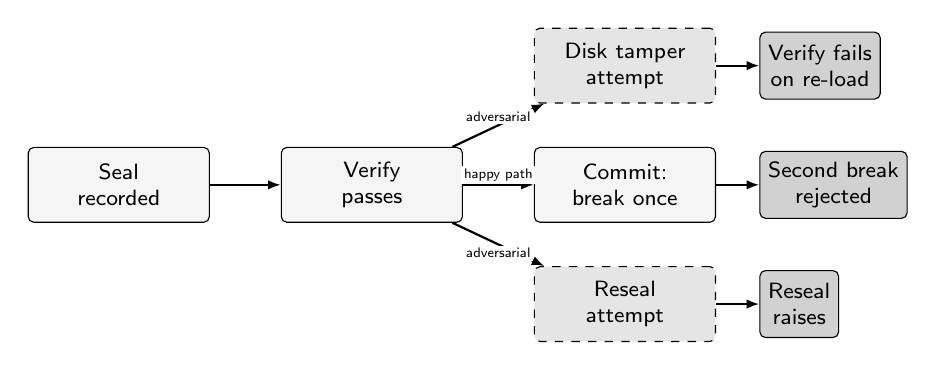
\begin{tikzpicture}[
  font=\footnotesize\sffamily,
  ok/.style={draw, rounded corners=2pt, align=center,
    inner sep=4pt, minimum height=0.95cm, minimum width=2.3cm,
    fill=black!4},
  adv/.style={draw, rounded corners=2pt, align=center,
    inner sep=4pt, minimum height=0.95cm, minimum width=2.3cm,
    fill=black!10, dashed},
  fail/.style={draw, rounded corners=2pt, align=center,
    inner sep=3pt, minimum height=0.85cm, fill=black!18},
  arr/.style={-{Latex[length=1.6mm]}, thick},
  lbl/.style={font=\tiny\sffamily, fill=white, inner sep=1pt}
]
  % main flow
  \node[ok] (s1) {Seal\\recorded};
  \node[ok, right=0.9cm of s1] (s2) {Verify\\passes};

  % 3 paths out of verify-OK (audit forks)
  \node[adv, above right=0.55cm and 0.9cm of s2] (s3) {Disk tamper\\attempt};
  \node[fail, right=0.55cm of s3] (s4) {Verify fails\\on re-load};

  \node[ok, right=0.9cm of s2] (s5) {Commit:\\break once};
  \node[fail, right=0.55cm of s5] (s6) {Second break\\rejected};

  \node[adv, below right=0.55cm and 0.9cm of s2] (s7) {Reseal\\attempt};
  \node[fail, right=0.55cm of s7] (s8) {Reseal\\raises};

  \draw[arr] (s1) -- (s2);
  \draw[arr] (s2) -- (s3) node[lbl, midway, above] {adversarial};
  \draw[arr] (s3) -- (s4);
  \draw[arr] (s2) -- (s5) node[lbl, midway, above] {happy path};
  \draw[arr] (s5) -- (s6);
  \draw[arr] (s2) -- (s7) node[lbl, midway, below] {adversarial};
  \draw[arr] (s7) -- (s8);
\end{tikzpicture}
\caption{Seal lifecycle paths exercised by \code{scripts/reproduce\_seal\_demo.py}.
  \code{verify} after seal creation returns the canonical-OK state; from there,
  three audit forks are explored: an on-disk tamper attempt (verify fails),
  the happy-path commit (single break succeeds, second break is rejected), and
  a reseal attempt on a still-sealed file (raises).  Adversarial forks use a
  dashed style; success nodes are filled lightly; failure endpoints are darker.
  The micro-demo uses a temporary seal file and fixed digest; it does not open
  registered-experiment holdouts or touch \code{data\_cache/}.}
\label{fig:seal}
\end{figure}

\begin{figure}[t!]
\centering
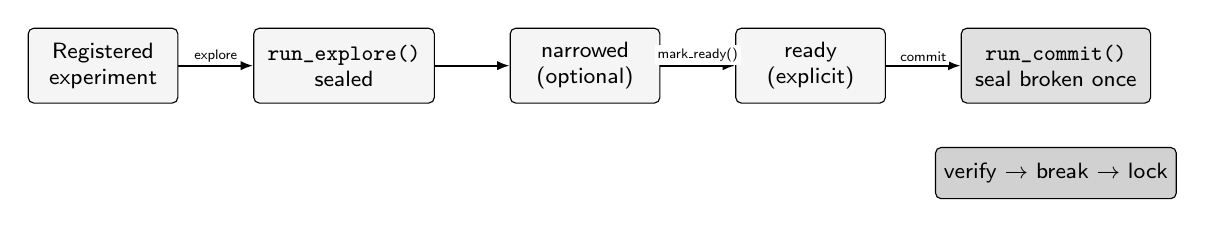
\begin{tikzpicture}[
  font=\footnotesize\sffamily,
  stage/.style={draw, rounded corners=2pt, align=center,
    inner sep=5pt, minimum height=0.95cm, minimum width=1.9cm,
    fill=black!4},
  gateok/.style={draw, rounded corners=2pt, align=center,
    inner sep=3pt, minimum height=0.65cm, fill=black!10},
  arr/.style={-{Latex[length=1.6mm]}, thick},
  lbl/.style={font=\tiny\sffamily, fill=white, inner sep=1pt}
]
  \node[stage] (e1) {Registered\\experiment};
  \node[stage, right=0.95cm of e1] (e2) {\fct{run\_explore}\\sealed};
  \node[stage, right=0.95cm of e2] (e3) {narrowed\\(optional)};
  \node[stage, right=0.95cm of e3] (e4) {ready\\(explicit)};
  \node[stage, right=0.95cm of e4, fill=black!12] (e5) {\fct{run\_commit}\\seal broken once};

  \draw[arr] (e1) -- (e2) node[lbl, midway, above] {explore};
  \draw[arr] (e2) -- (e3);
  \draw[arr] (e3) -- (e4) node[lbl, midway, above] {mark\_ready()};
  \draw[arr] (e4) -- (e5) node[lbl, midway, above] {commit};

  % seal gate indicator under commit
  \node[gateok, below=0.55cm of e5, fill=black!18] (g1) {verify $\to$ break $\to$ lock};
\end{tikzpicture}
\caption{Explore / commit lifecycle for a registered experiment.
  Only \fct{run\_commit} (rightmost stage) breaks the seal after
  \code{verify()} passes; a broken seal cannot be re-sealed, and
  re-running \fct{run\_explore} does not consume the holdout.}
\label{fig:workflow}
\end{figure}

On \code{ResearchSession} construction the package loads holdout-range inputs
from the data cache and computes a SHA256 digest.  The hasher lives at
\code{\_compute\_holdout\_data\_hash} in the session module
(see the module-path lists at the start of each tool description and in Section~\ref{sec:capabilities}).
Let $\mathcal{S}$ be the sorted symbol set.  For each $s\in\mathcal{S}$ the
hasher feeds a CSV serialization of every present column (open, high, low,
close, volume) with no row index.
Hashing the full OHLCV row rather than just close detects tampering on
path-dependent stops or volume-driven features.  Extended-history frames used
for EMA warmup at commit time are hashed under the same column rule.
If funding series are present, each symbol contributes \code{time} and
\code{funding\_rate} columns because funding enters trade PnL in the engine.
The digest is therefore a fingerprint of every input that can change holdout
scores under the package's feature and cost model.

\paragraph{Seal record and authentication.}
The digest is written into a seal object (\code{HoldoutSet} in
\code{audit/holdout.py}) with holdout start and end dates, a UTC sealed-at
timestamp, an optional broken-at time, and an HMAC-SHA256 signature.  The seal
file is JSON.  The MAC uses a canonical serialization with sorted keys and
tight separators, excluding the signature field and the local path so that
moving the file does not invalidate an otherwise intact seal.  The secret is
read only from \code{QUANT\_LIB\_HMAC\_SECRET} (minimum 32 characters); there
is no insecure default.  Verification uses constant-time comparison
(\code{hmac.compare\_digest}).  Post-signature checks match the stored data
hash and detect a prior break.

\paragraph{Workflow invariants.}
\begin{enumerate}
  \item \fct{run\_explore} builds the session with
    \code{\_skip\_holdout\_load=True} so the public explore path never
    materializes holdout features for scoring; the seal is not broken.
  \item \fct{run\_commit} requires candidate stage \code{ready}, checks
    \code{is\_sealed()} and \code{verify()}, recomputes the SHA256 from the
    session's cached holdout, BTC-extended, and funding payloads, and aborts on
    mismatch before any holdout trades are scored.
  \item \code{commit\_break} re-verifies disk state, then writes
    \code{broken\_at}, the post-break \code{data\_hash}, and a fresh HMAC in a
    single save.  A broken seal cannot be re-sealed; a later session against the
    same seal path loads the prior broken state when the signature remains valid
    under the current secret.
\end{enumerate}
The cryptographic primitives are standard.  What is package-specific to the sealed-holdout path is the
session-level wiring: hash coverage, one-shot break, and the explore/commit
split that keeps paper-grade SPA replication explore-only.  Audit-process instruments
(Subsection~\ref{sssec:au-hypo}) pre-date the seal and supply the registered
experiment bindings that anchor each \code{HoldoutSet} to a named strategy.

\paragraph{Replication micro-demo (Claim~1).}
The SPA path under \code{replication/output\_paper\_grade/} never opens a
registered-experiment holdout.  A separate synthetic script exercises
Claim~1 for reviewers: \code{scripts/reproduce\_seal\_demo.py}, runnable
via \code{make reproduce-seal}.

The script seals a temp JSON holdout, then verifies it.  It tampers the
on-disk \code{data\_hash} so \code{verify()} fails.  It runs
\code{commit\_break} once and checks one-shot invariants (second break
fails, reseal raises).  The committed cross-check sample lives under
\code{replication/output\_seal\_demo/}.  That path does not score market
trades and does not call \fct{run\_commit} on paper experiments.


\subsection{Probabilistic Sharpe Ratio on engine returns}
\label{subsec:claim-psr}

\citet{Bailey+LopezDePrado:2012,Bailey+LopezDePrado:2014} define and develop the
Probabilistic Sharpe Ratio as the probability that the true Sharpe ratio exceeds
a benchmark after adjusting for estimation error under non-normal returns.  With
sample Sharpe $\widehat{\mathrm{SR}}$, benchmark $\mathrm{SR}^*$, sample size
$n$ (or effective sample size $n_{\mathrm{eff}}$), skewness $\gamma_3$, and
regular kurtosis $\gamma_4$,
\begin{equation}
  \widehat{\mathrm{PSR}}
  =
  \Phi\!\left(
    \frac{\widehat{\mathrm{SR}}-\mathrm{SR}^*}
         {\sqrt{\widehat{V}/(n_{\mathrm{eff}}-1)}}
  \right),
  \quad
  \widehat{V}
  =
  1 - \gamma_3\,\widehat{\mathrm{SR}}
    + \frac{\gamma_4-1}{4}\,\widehat{\mathrm{SR}}^2.
\end{equation}
With excess kurtosis $\kappa=\gamma_4-3$ (Fisher convention as in
\pkg{scipy.stats.kurtosis}), the kurtosis term equals $(\kappa+2)/4$.  The same
variance-of-SR structure appears in the deflated-Sharpe construction discussed
in Subsection~\ref{subsec:additional-stats}.

Function \code{prob\_sharpe\_ratio} in \code{quant\_lib/core/\_testing.py}
implements that formula on a one-dimensional return array.
\begin{itemize}
  \item Unweighted path: sample mean and sample standard deviation
    (\code{ddof=1}), denominator $n-1$, return $(\mathrm{NaN},\mathrm{NaN})$ if
    $n<10$, zero variance, or non-finite extreme SR.
  \item Weighted path: weighted mean and variance after normalizing weights to
    sum to one. Kish ESS \citep{Kish:1965}
    $n_{\mathrm{eff}}=1/\sum_i w_i^2$; reject if $\mathrm{ESS}<2$.
  \item Optional annualization multiplies SR (and rescales the benchmark) by
    $\sqrt{365.25}$ for daily series.  Commit-time trade PSR disables
    annualization because inputs are per-trade $R$-multiples, not daily
    returns.
  \item Variance correction is clipped to a small positive floor when Bailey's
    asymptotic expansion leaves the valid range (very high SR with near-normal
    higher moments), so callers receive a usable PSR near one rather than a
    silent NaN from a negative variance term.
\end{itemize}
Skewness and excess kurtosis are computed with \pkg{scipy.stats}.  The WFA
in-sample objective reuses the same Bailey variance correction so search and
reporting share one formula family (Subsection~\ref{subsec:claim-wfa}).

\paragraph{Explore versus commit.}
\fct{run\_explore} never opens the seal and therefore does not return the holdout
PSR.  Paper-grade \code{scripts/reproduce.py} is explore-only and reports SPA
and trade counts.  Holdout PSR is computed in
\code{quant\_lib/research/commit.py} on executed holdout $R$-multiples after
seal break.  Reviewers comparing manuscript tables to the public explore path
should not expect a holdout PSR column.

\paragraph{Relation to supporting tools.}
The PSR surface reuses the Kish ESS gate from
Subsection~\ref{sssec:pr-ess} and shares its variance-of-SR term with the
deflated Sharpe computation in Subsection~\ref{sssec:sl-dsr}.  Both pieces
consume the same \code{prob\_sharpe\_ratio} return tuple so that commit-time
PSR and deflated Sharpe never disagree on higher moments of the trade series.

\subsection{SPA with dual null constructions}
\label{subsec:claim-spa}

\citet{Hansen:2005} SPA tests whether the best of $K$ competing rules has
superior predictive ability relative to a benchmark, with studentization and
recentering that improve behavior when many poor alternatives are present.
\citet{White:2000} supplies the related reality-check background.  Finite-sample
Monte Carlo $p$-values use the Phipson--Smyth add-one form
\begin{equation}
  p = \frac{1 + \#\{\mathrm{null}\ge\mathrm{obs}\}}{B+1}
\end{equation}
so $p$ cannot be zero under random draws \citep{Phipson+Smyth:2010}.

\paragraph{Shared entry point.}
\code{portfolio\_spa} in \code{quant\_lib/core/\_spa.py} is the single SPA
entry.  Callers pass observed out-of-sample trade dicts (including
\code{r\_net}, times, symbol, and stop parameters), per-symbol asset panels,
daily close and high/low matrices, portfolio risk knobs, and iteration budget
$B$ (\code{n\_iters}; paper default $B=2000$ via \fct{run\_explore}).  Two null
constructions coexist.  The public edge path evaluates both and stores both
$p$-values.

\begin{figure}[t!]
\centering
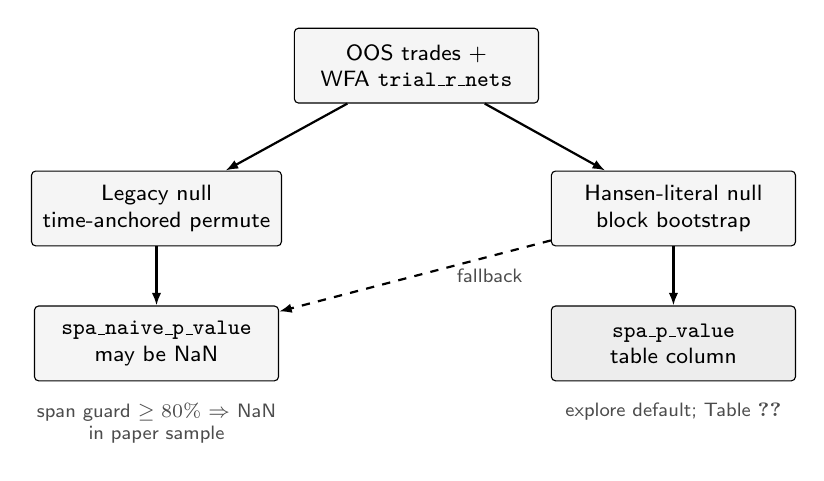
\begin{tikzpicture}[
  font=\footnotesize\sffamily,
  box/.style={draw, rounded corners=1.5pt, align=center,
    inner sep=4pt, minimum height=0.95cm, minimum width=3.1cm,
    fill=black!4},
  arr/.style={-{Latex[length=1.6mm]}, thick},
  note/.style={font=\scriptsize\sffamily, text=black!70, align=center}
]
  \node[box] (in) {OOS trades +\\WFA \texttt{trial\_r\_nets}};
  \node[box, below left=0.85cm and 0.15cm of in] (leg) {Legacy null\\time-anchored permute};
  \node[box, below right=0.85cm and 0.15cm of in] (han) {Hansen-literal null\\block bootstrap};
  \node[box, below=0.75cm of leg] (pn) {\texttt{spa\_naive\_p\_value}\\may be NaN};
  \node[box, below=0.75cm of han, fill=black!7] (ph) {\texttt{spa\_p\_value}\\table column};

  \draw[arr] (in) -- (leg);
  \draw[arr] (in) -- (han);
  \draw[arr] (leg) -- (pn);
  \draw[arr] (han) -- (ph);
  \draw[arr, dashed] (han) -- node[note, midway, right=0.05cm, xshift=0.35cm]
    {fallback} (pn);

  \node[note, below=0.15cm of pn]
    {span guard $\ge 80\%$ $\Rightarrow$ NaN\\in paper sample};
  \node[note, below=0.15cm of ph]
    {explore default; Table~\ref{tab:spa}};
\end{tikzpicture}
\caption{Dual-null SPA wiring on the explore path.  Both $p$-values are
  stored; Table~\ref{tab:spa} reports Hansen-path \code{spa\_p\_value}.
  Legacy NaN under the anchor-span guard is intentional, not a failed run.}
\label{fig:spa-dual}
\end{figure}

\paragraph{Legacy null (always computed).}
The legacy null preserves cross-asset co-occurrence by time-anchored circular
permutation of the observed trade set:
\begin{enumerate}
  \item Simulate observed portfolio equity $E_{\mathrm{obs}}$ with
    \code{simulate\_full\_portfolio} under the same leverage, margin,
    position-limit, and circuit-breaker settings as the live path.
  \item Record each trade's hour offset from the first entry and its duration.
  \item For $b=1,\ldots,B$, draw a uniform anchor in the global hour span,
    remap every trade entry by modular arithmetic on the symbol timeline,
    re-simulate exits under the same WFA cost model (fees, weekend penalty,
    stress multiplier), then re-run the portfolio simulator to obtain $E_b$.
    Exit re-simulation uses the package trailing-stop helper.
  \item Set
    $p_{\mathrm{naive}}=(1+\#\{E_b\ge E_{\mathrm{obs}}\})/(B+1)$.
\end{enumerate}
Degenerate guards return non-misleading sentinels: empty trade list $\to p=1$;
NaN observed equity $\to p=\mathrm{NaN}$; all null equities stuck at initial
capital $\to p=1$; anchor span at least $80\%$ of the calendar $\to$ legacy
$p=\mathrm{NaN}$ (null nearly identical to the observed path).
In the paper-grade explore sample under
\code{replication/output\_paper\_grade/}, the stored
\code{spa\_naive\_p\_value} fields are $\mathrm{NaN}$ for all three
strategies under that anchor-span guard, while
\code{spa\_p\_value} remains the Hansen-literal $p$ (or Hansen's
fallback to the legacy $p$ when Hansen cannot run).  Table~\ref{tab:spa}
therefore reports Hansen-path \code{spa\_p\_value} only; a NaN legacy
field is an intentional guard output, not a failed SPA run.
Legacy $p$ is finite when the remapped trade anchor span is under the
$80\%$ calendar threshold---typically shorter evaluation windows, lighter
lookbacks, or denser bars relative to trade duration---so dual storage is
not redundant outside this sample.  Explore defaults still treat
Hansen-path \code{spa\_p\_value} as the primary reported column.


\paragraph{Hansen-literal null (explore default).}
When the recenter policy is Hansen-literal, statistics are returned, and WFA
supplies non-empty per-trial in-sample PnL arrays (\code{trial\_r\_nets}), a
NumPy-only Hansen helper runs without calling the trade simulator.  Legacy
permutation RNG streams stay untouched. Hansen uses a separate generator seeded
at \code{seed+1}.  Under a zero-mean benchmark, loss differentials are
$d_k=-r_{\mathrm{net},k}$.  For each trial $k$ and bootstrap draw $b$,
stationary block resampling of $d_k$ \citep{Politis+Romano:1994} with expected
block length $p_k=\max(1,\mathrm{round}(n_k^{1/3}))$ (or a static override)
yields studentized statistics
\[
  T^{k}_{b}
  =
  \sqrt{n_k}\,\bar d^{k}_{b}/\widehat{\sigma}(d_k).
\]
Hansen Equation~7 recentering discards negative-mean bootstrap statistics;
Equation~8 takes the cross-trial maximum
$T^{\mathrm{null}}_b=\max_k T^{k,\mathrm{acc}}_b$.  The observed statistic uses
the out-of-sample winner's $r_{\mathrm{net}}$ the same way.  Then
\[
  p_{\mathrm{hansen}}
  =
  \bigl(1+\#\{T^{\mathrm{null}}_b\ge T_{\mathrm{obs}}\}\bigr)/(B+1).
\]
On missing trials, $N_{\mathrm{obs}}<2$, or zero-variance series, Hansen falls
back to the legacy $p$ and records \code{fallback=True}.

\code{Candidate.run\_edge\_testing} aggregates \code{trial\_r\_nets} from every
WFA fold, calls \code{portfolio\_spa} with Hansen kwargs, and stores
\begin{itemize}
  \item \code{spa\_p\_value} $=p_{\mathrm{hansen}}$ (or legacy on fallback);
  \item \code{spa\_naive\_p\_value} $=p_{\mathrm{naive}}$.
\end{itemize}
Paper Table~\ref{tab:spa} reports the explore-path \code{spa\_p\_value} at
$B=2000$.  The public thin wrapper \code{tools.stats.spa\_test} exposes the
legacy three-tuple API; paper-grade numbers come from the explore pipeline's
Hansen settings, not from inventing a different null in that wrapper.

\paragraph{Relation to supporting tools.}
The SPA null construction runs against the same portfolio equity path that the
cost accounting layer (Subsection~\ref{sssec:co-costs}) builds, so a reviewer
auditing the legacy permutation can trace every per-trade cost component
from engine to null.  Across the registered-experiment family, the
Bonferroni / journal counter (Subsection~\ref{sssec:mt-journal}) reports
$n_{\mathrm{tests}}$ and $\alpha_{\mathrm{adj}}$ beside the SPA $p$ so the
explore table can be read alongside its family-level multiplicity context.
The FDR step-up (Subsection~\ref{sssec:mt-fdr}) is intentionally not applied
to the paper Table because the three SPA $p$-values are a fixed,
pre-registered family and applying FDR would only rescale them toward one
without changing the rejection set.

\paragraph{Hansen-fallback diagnostics.}
When Hansen cannot run, either because \code{trial\_r\_nets} is missing, because
fewer than two observed trades survive, or because trial or observed series are
zero-variance, the explore path records
\code{hansen\_fallback = True} on the candidate
\code{edge\_metrics} object and returns the legacy $p$ in place of
$p_{\mathrm{hansen}}$.
\code{spa\_naive\_p\_value} remains the legacy circular-permutation $p$ in
the same return object.  In the paper-grade explore sample under
\code{replication/output\_paper\_grade/}, the published
\code{spa\_p\_value} columns are Hansen-path values (no fallback substitution
into the table), while \code{spa\_naive\_p\_value} stays $\mathrm{NaN}$ for all
three strategies under the legacy anchor-span guard.  Reviewers can confirm the
two SPA $p$ fields from \code{results.json} without re-running the SPA
pipeline; the boolean fallback flag itself is an in-process
\code{edge\_metrics} diagnostic rather than a top-level sample key.

\paragraph{Worked numerical trace.}
To make the formulas auditable without re-running the pipeline, the
paper-grade sample under \code{replication/output\_paper\_grade/}
records the three SPA columns together with their underlying counts.
At \code{n\_spa\_iters} $= B = 2000$, the Phipson--Smyth add-one form
$p_{\mathrm{hansen}} = (1 + \#\{T^{\mathrm{null}}_b \ge T_{\mathrm{obs}}\})/(B+1)$
imply the bootstrap exceedance count $\#\{T^{\mathrm{null}}_b \ge T_{\mathrm{obs}}\}$
directly:

\begin{table}[h!]
\centering
\begin{tabular}{lrrr}
\toprule
Strategy & $T_{\mathrm{obs}}$ exceedance & $p_{\mathrm{hansen}}$ & $p_{\mathrm{naive}}$ \\
\midrule
\code{vol\_compression\_v1}    & $2000$ & $1.0000$ & $\mathrm{NaN}$ \\
\code{pullback\_sniper\_rsi}   & $1860$ & $0.9300$ & $\mathrm{NaN}$ \\
\code{funding\_rate\_carry}    & $\phantom{0}0$ & $0.0005$ & $\mathrm{NaN}$ \\
\bottomrule
\end{tabular}
\caption{SPA $p$-values and implied bootstrap exceedance counts at
  $B = 2000$.  Phipson--Smyth add-one prevents an exact zero
  ($p = 1/(B+1) = 1/2001 \approx 0.0005$) so the FRC reject is
  $\#\{\mathrm{null}\ge\mathrm{obs}\} = 0$, not a zero-cell artefact.
  The legacy circular-permutation column stays $\mathrm{NaN}$ for all
  three strategies under the $80\%$ calendar-span guard; the table is
  the explore-path Hansen column only.}
\label{tab:spa-exceed}
\end{table}

\paragraph{H\(_0\) sanity simulation.}
A reviewer audit can ask whether the dual-null + Hansen-literal
implementation produces non-degenerate $p$-values under the null.
We ran an off-band sanity simulation: $K = 5$ trial series of
$n = 60$ zero-mean Gaussian returns ($\sigma = 0.01$) and an
independent observed series, re-using
\code{quant\_lib.core.\_spa.\_hansen\_spa\_p\_value} at $B = 500$.
Eight independent replications yielded $p \in \{0.477, 0.998, 0.257,
0.946, 0.910, 0.465, 0.273, 0.255\}$ with mean $0.573$, median $0.471$,
and zero rejections at $\alpha = 0.10$.  This is informal (small $B$
and small $K$); the package does not publish a calibration table
because a numerical-statistics calibration paper is out of scope.
What the simulation does establish is that the implementation does
not collapse to $p = 0$ or $p = 1$ on every call, so reviewers
auditing the boundary behaviour can interpret the in-sample SPA
numbers with confidence.

\paragraph{Finite-sample divergences and disclosures.}
Relative to a strict reading of Hansen's asymptotic SPA setup, the
Hansen-literal path discloses four finite-sample choices that the
implementation does \emph{not} silently ``fix'':
(i)~expected block length is the Politis--Romano rule
$p=\max(1,\mathrm{round}(n_k^{1/3}))$ per trial (or a fixed override via
\code{STATIC["spa\_hansen\_block\_length\_override"]}), without automatic
Patton--Politis--White block selection;
(ii)~trial lengths $n_k$ may differ across Optuna trials, and the path does
not apply a $\sqrt{N/n_k}$ sample-size rescale;
(iii)~Hansen's two-stage $q$ bootstrap (Hansen 2005, Section~3) is omitted---the
Eq.~7 recenter plus Eq.~8 max-statistic is the data-snooping correction used
here;
(iv)~finite-sample uniformity of the max-of-$K$ null is an empirical
calibration statement at finite $B$ and $n_k$, not an asymptotic theorem.
Two sample-path guards sit beside those divergences and are visible in the
paper-grade explore artifacts: the legacy circular permutation returns
$\mathrm{NaN}$ when the anchor span is at least $80\%$ of the calendar, and
the Hansen path substitutes the legacy $p$ with
\code{hansen\_fallback = True} on zero-variance or singleton inputs (not
triggered for the published table).  Both $p$-values use the Phipson--Smyth
add-one form, so a published $p\approx 0.0005$ at $B=2000$ reflects
$\#\{\mathrm{null}\ge\mathrm{obs}\}=0$, not a zero-cell artefact.  Monte Carlo
standard error is $\mathcal{O}(1/\sqrt{B})$; paper-grade results fix
$B=2000$ and reviewers should not down-sample.


\subsection{Deterministic walk-forward analysis}
\label{subsec:claim-wfa}

Walk-forward analysis optimizes on rolling or expanding in-sample windows,
evaluates the next out-of-sample block, and advances \citep{Pardo:2008}.  Purge
gaps reduce boundary leakage from long-lookback features.  The package does not
invent WFA; it engineers a seedable, recorded realization integrated with seal,
SPA, and risk allocation.

\code{run\_wfa\_per\_symbol} in \code{quant\_lib/core/\_wfa.py} sorts months per
eligible symbol.  Folds use expanding in-sample history from
\code{wfa\_min\_train\_months} with out-of-sample length
\code{wfa\_test\_months}.  Adaptive purge days shrink with longer in-sample
history (90 / 60 / 30 days by in-sample month buckets) via
\code{\_get\_purge\_days}.  Folds with too few bars or gaps larger than
\code{max\_allowed\_gap\_hours} are skipped.  The per-fold seed is
\[
  \texttt{fold\_seed}
  =
  \texttt{GLOBAL\_SEED}
  \oplus \sum_c \mathrm{ord}(c)
  \oplus (y\cdot 100 + m),
\]
where the sum is over characters of the symbol ticker and $(y,m)$ is the last
in-sample month.  Independent RNG streams for Optuna warm-start perturbation,
out-of-sample cost noise, and in-sample cost noise use fixed XOR masks on that
seed (\code{0xDEF}, \code{0xABCD}, \code{0xBEEF}).

Each fold runs \pkg{Optuna} \code{TPESampler(seed=fold\_seed)}
\citep{Akiba+etal:2019} with an adaptive trial budget.  \code{WalkForwardObjective}
suggests strategy parameters from the experiment search space, runs the
\pkg{Numba} \code{fast\_trade\_loop} \citep{Lam+etal:2015} on purged in-sample
bars, and scores a PSR-style objective with time-decay bar weights (halflife in
months), Kish ESS trade reweighting \citep{Kish:1965}, optional L2 pull toward
parameter centers, and a log-ESS trade-count weight.  Early exits (too few
bars/trades, non-positive weighted variance) return a large negative score and
append a \code{None} sentinel to \code{trial\_r\_nets}; successful trials append
the in-sample PnL array consumed later by Hansen SPA.

Winning parameters are frozen per fold; out-of-sample trades are generated with
the same engine and fold-specific cost RNG.  Fold metadata records best
parameters, objective value, and the full \code{trial\_r\_nets} list
(JSON-friendly lists so reproducibility equality tests remain unambiguous).
Across symbols, \code{Candidate.run\_edge\_testing} concatenates out-of-sample
trades, picks per-symbol frozen parameters by best fold PSR, applies
profit-factor-weighted risk allocation preferably from in-sample trades
(decoupled from the out-of-sample SPA sample; see
Subsection~\ref{subsec:additional-stats}), simulates the portfolio, then runs
SPA as in Claim~3.

Reviewers should check determinism (same experiment name, data, and seeds
reconstruct the same fold path), purge policy, and the explicit handoff of
in-sample trial PnL into Hansen SPA; not a new theory of walk-forward testing.

\paragraph{Relation to supporting tools.}
The WFA in-sample objective reuses the Kish ESS gate from
Subsection~\ref{sssec:pr-ess} so that search cannot manufacture precision
with degenerate weighting.  Across folds, the PF-weighted risk allocator
(Subsection~\ref{sssec:au-pf}) takes the per-fold
\code{trial\_r\_nets} list as input, runs halflife-decayed PF weighting on
the IS trade pool, and returns a final symbol-risk dict that the portfolio
simulator resizes.  Together with Claim~3, this closes the chain
WFA IS trials $\rightarrow$ Hansen SPA inputs $\rightarrow$ portfolio
equity $\rightarrow$ costed $R$-multiples used in Claim~2.

\subsection{Additional statistical and process tools}
\label{subsec:additional-stats}

The four primary claims do not exhaust the statistical surface of \pkg{quant\_lib}.  This subsection documents the supporting tools that ship with the package, the formulas they implement, the code paths that wire them to the explore and commit pipelines, and how each tool relates to the primary claims.  Eleven supporting tools are grouped into five clusters: multi-test accounting (\ref{sssec:mt-fdr}, \ref{sssec:mt-journal}), selection-inflation control (\ref{sssec:sl-dsr}, \ref{sssec:sl-label}), path-risk quantification (\ref{sssec:pr-bootstrap}, \ref{sssec:pr-ess}), audit and process instrumentation (\ref{sssec:au-hypo}, \ref{sssec:au-pf}), and cost / engine realism (\ref{sssec:co-costs}, \ref{sssec:co-facade}).  Each entry is treated at medium depth, enough for a reviewer to locate, audit, and reproduce the implementation by following the named module.  Source-of-truth module paths are inline at the start of each tool's description.

\subsubsection{Multi-test accounting}
\label{sssec:mt-fdr}

\paragraph{Benjamini--Hochberg FDR correction.}  Given an unordered vector of raw $p$-values $p_1, \ldots, p_n$ with significance target $\alpha$, \citet{Benjamini+Hochberg:1995} replace the family-wise Bonferroni bound by the step-up procedure: sort $p$ ascending into $p_{(1)} \le \ldots \le p_{(n)}$, find the largest $k$ such that $p_{(k)} \le k\alpha/n$, and reject all hypotheses with $p \le p_{(k)}$.  Adjusted $q$-values follow as $q_{(i)} = \min_{j \ge i} \, p_{(j)} j/n$ (right-to-left cumulative minimum) so monotone non-decreasingness is preserved.  Function \code{fdr\_correction} in \code{quant\_lib/core/\_testing.py} returns the tuple \code{(reject\_mask, q\_values)}; the CLI alias \code{fdr\_correct} in \code{quant\_lib/tools/stats.py} re-exports it for notebook and \code{quant\_exp} callers.  The result drives Table-level FDR columns only when the table has more than a handful of cells; the paper Table~\ref{tab:spa} is left raw because the three SPA $p$-values form a fixed, pre-registered family and FDR would just rescale them toward one with no new inferences.

\label{sssec:mt-journal}

\paragraph{Bonferroni context and the experiment journal.}  Multiplicity across an entire research program is the count of registered experiments that have been pushed through the machine, not the row count of one Table.  The \code{ExperimentLog} class in \code{quant\_lib/audit/journal.py} threads a registry counter across every \code{run\_explore} / \code{run\_commit} call: \code{log\_run(description, category, params\_snapshot)} appends a structured entry and \code{n\_tests} returns a credit-weighted count
\[
  n_{\mathrm{tests}} = n_{\mathrm{experiments}} + 0.5 \cdot n_{\mathrm{ablations}},
\]
which feeds the next-test adjusted significance level
\[
  \alpha_{\mathrm{adj}} = \alpha_0 / (n_{\mathrm{tests}} + 1).
\]
Bugfix entries are logged but excluded from the counter, so a fix-up round does not inflate multiplicity.  The +1 in the denominator avoids division-by-zero before any experiment has been run.  The CLI report layer prints Bonferroni and FDR context fields beside SPA so the reviewer sees the multiplicity state without opening the journal file.

\subsubsection{Selection-inflation control}
\label{sssec:sl-dsr}

\paragraph{Deflated Sharpe Ratio.}  When the in-sample optimizer is Optuna and the search space contains many trial configurations, the family size $N$ that matters for selection inflation is the Optuna search budget, not the registered-experiment count.  \citet{Bailey+LopezDePrado:2014} derive the deflated Sharpe probability
\[
  \mathrm{DSR} = \Phi\bigl( (\widehat{S} - S_{\max}) \sqrt{ \frac{n-1}{1 - \gamma_1 \widehat{S} + \frac{\gamma_2 - 1}{4} \widehat{S}^2} } \bigr),
\]
where $\widehat{S}$ is the observed Sharpe, $S_{\max} \approx \sqrt{2 \ln N} - \frac{\ln(\ln N) + \ln(4\pi)}{2 \sqrt{2 \ln N}}$ approximates the expected maximum of $N$ null Sharpes via the normal tail quantile, and $\gamma_1$, $\gamma_2$ are skewness and excess kurtosis of the trade $R$-multiple series.  Function \code{deflated\_sharpe\_ratio} in \code{quant\_lib/core/\_testing.py} accepts \code{(observed\_sr, n\_trials, skew, excess\_kurt, n\_observations\_per\_trial=None)} and returns $\mathrm{DSR} \in [0,1]$; the implementation returns $\mathrm{NaN}$ when $N<2$ (no multiple testing) and $0$ when the observed Sharpe does not beat $S_{\max}$.  Commit reporting attaches DSR when the family size is known; the explore-only paper Table~\ref{tab:spa} centers SPA because SPA already wraps $N$ trials into its own null.

\paragraph{DSR position relative to the paper case-study sample.}
For the three case studies, the Optuna in-sample trial budget that feeds PSR / SPA is the adaptive trial count returned by the WFA fold objective, not a fixed $N$.  The framework's WFA target is a TPE search that returns when the best objective stalls; the actual $N_{\mathrm{trials}}$ per fold varies across folds and symbols.  Two consequences.  First, a paper-grade DSR row in Table~\ref{tab:spa} would need a fold-aggregated $N$ definition (e.g., the union of trial configurations across folds and symbols), and the package does not yet expose that aggregate in the explore pipeline.  Second, the cost of committing DSR alongside SPA in the explore sample is the cost of re-running the portfolio with both allocators and saving the raw $R$-multiples, neither of which is in the committed sample.  We therefore disclose DSR at formula and signature level in this paper and report DSR alongside PSR at commit time (where the trade $R$-multiple series is available); a single-shot explore sample without commit-time $R$-multiples cannot produce DSR honestly.

\label{sssec:sl-label}

\paragraph{P-value labeling.}  The CLI, HTML report layer, and PDF output all read $p$-values from the same \code{ExploreResult} objects.  A reviewer cross-checking them should not be told that $p=0.93$ is ``inconclusive'' on one page and ``non-rejecting'' on another.  Function \code{label\_p\_value} in \code{quant\_lib/core/\_testing.py} takes \code{(p, context)} (where \code{context} is one of \code{"mean\_r"}, \code{"spa"}, or \code{"bonferroni"}) and returns a triple \code{(category\_label, strength\_label, prose\_label)} keyed at $\alpha=0.05$:
"strong reject" for $p<0.01$, "reject" for $p<0.05$, "borderline" for $p<0.10$, and "non-reject" for $p \ge 0.10$.  Numeric $p$ stays byte-identical across PDF, terminal, and notebooks.  Only the wording is centralized.

\subsubsection{Path-risk quantification}
\label{sssec:pr-bootstrap}

\paragraph{Bootstrap helpers for path risk.}  Whether the realised $R$-multiples are statistically superior is one question; whether the same path survives resampling is another.  Circular block bootstrap on a trade- or day-return series with expected block length $b$ approximates the sampling distribution of CAGR and maximum drawdown without assuming independence.  Function \code{bootstrap\_daily\_returns} in \code{quant\_lib/core/\_metrics.py} picks a block length under the \citet{Politis+Romano:1994} rule $\widehat{b} = \bigl(\,\lfloor 3.15\, n^{1/3}\rfloor,\,\lceil 1.5\, n^{1/3}\rceil \,\bigr)$ so the polling bias is small relative to the asymptotic-variance estimate; for sparse trade series \code{bootstrap\_trade\_multiples} resamples blockwise over the $R$-multiple list with the same expected block length.

\paragraph{Block length chosen for the paper sample.}
Applying $\widehat{b} = \mathrm{round}(n_{\mathrm{trades}}^{1/3})$ to the three case-study samples gives $\widehat{b} = 8$ for \code{vol\_compression\_v1} ($n_{\mathrm{trades}} = 438$), $\widehat{b} = 6$ for \code{pullback\_sniper\_rsi} ($n_{\mathrm{trades}} = 180$), and $\widehat{b} = 15$ for \code{funding\_rate\_carry} ($n_{\mathrm{trades}} = 3446$).  The Hansen SPA path reuses the same Politis--Romano rule per trial and operates on the same $n_k^{1/3}$ scaling, so bootstrap and SPA share a single block-length convention.  In denser trade series such as funding-rate carry, $\widehat{b}$ grows sub-linearly with $n$ ($3446^{1/3} \approx 15$), keeping the number of effective blocks $n / \widehat{b}$ large enough for the asymptotic-variance approximation to hold.  Daily bootstrap pads each zero-return day as a no-trade day at block boundaries, which inflates sample size and biases path-risk estimates; trade block bootstrap is the default on \code{CommitResult} when the number of trades is much smaller than the number of calendar bars.  Both helpers reuse the Politis--Romano block primitives already used inside Hansen SPA; they are not substitutes for Claim~3's dual null.

\label{sssec:pr-ess}

\paragraph{Kish effective sample size.}  When weights under time-decay (or any other uneven-exposure scheme) concentrate the mass on a few trades, the nominal sample size $n$ overstates precision.  \citet{Kish:1965} define the effective sample size of a non-negative weight vector $w$ as
\[
  n_{\mathrm{eff}} = \frac{(\sum_i w_i)^2}{\sum_i w_i^2} = \frac{1}{\sum_i \bar{w}_i^2}, \qquad \bar{w}_i = \frac{w_i}{\sum_j w_j},
\]
so uniform weights give $n_{\mathrm{eff}}=n$ and a single mass at one trade collapses to $n_{\mathrm{eff}}=1$.  The package does not expose a separate public \code{kish\_ess\_n} helper; Kish ESS is computed inline inside the weighted branch of \code{prob\_sharpe\_ratio} in \code{quant\_lib/core/\_testing.py} as $n_{\mathrm{eff}}=1/\sum_i w_i^2$ after weight normalization, and the same ESS gate rejects weighted-PSR formation when $n_{\mathrm{eff}}<2$.  The WFA in-sample objective reuses that weighted-PSR path, so search cannot manufacture precision with artificial weighting and the commit-time PSR surface shares one ESS definition.

\subsubsection{Audit and process instrumentation}
\label{sssec:au-hypo}

\paragraph{Hypothesis objects and pre-registration fields.}  A strategy that aspires to pre-registered evaluation needs declared mechanism, boundary conditions, and success criteria before it sees data.  \code{register\_hypothesis} (and the \code{Hypothesis} dataclass) in \code{quant\_lib/audit/hypothesis.py} puts that pre-registration into the code: it requires five narrative fields -- \code{name}, \code{mechanism}, \code{boundary\_conditions}, \code{success\_criteria}, and one of \code{entry\_logic} or \code{exit\_logic} -- and rejects blank or generic entries with a typed \code{HypothesisValidationError}.  A \code{QualityLevel} (\code{DRAFT}, \code{REVIEWED}, \code{REGISTERED}) flags whether the hypothesis is human-reviewed or machine-fast-tracked.  \code{experiments/} modules bind a strategy factory name plus these fields to a registered experiment on disk, so that \fct{run\_explore} can replay the same hypothesis + seed + universe triple that produced the original $p$-value.  This is an audit surface, not a statistical estimator, but it changes the way SPA inputs are interpreted because the success language is pre-committed.

\label{sssec:au-pf}

\paragraph{Profit-factor-weighted risk allocation.}  Across the universe, edge testing builds one portfolio from per-symbol OOS trades.  Equal-weight allocation is the naive choice; the package instead uses per-fold Profit Factor (PF) as a cheap meta-weight.  \code{apply\_pf\_weighted\_risk\_allocation} (and the IS-decoupled sibling \code{apply\_pf\_weighted\_risk\_allocation\_is}) in \code{quant\_lib/core/\_risk\_allocation.py} proceeds per OOS fold as follows.  Past folds contribute decay-weighted gross profit and loss with $d_{h}(n_{\mathrm{back}})=0.5^{n_{\mathrm{back}}/h}$, yielding a per-symbol PF.  That PF is mapped to a factor
\[
  f_j = \mathrm{clamp}\!\bigl(\mathrm{PF}_j,\; f_{\min},\; f_{\max}\bigr),
  \qquad f_{\min}=0.5,\; f_{\max}=1.5
\]
with those clamp defaults (or $1.0$ when past trade count is below a configured minimum; infinite-PF winners take $f_{\max}$).  Factors are then scaled by the baseline per-symbol risk and rescaled so the active-universe total risk budget is preserved (the X1 scheme).  Explore prefers the IS trade pool for past-fold PF when available, which removes the double-dipping failure mode that would arise if weight selection and SPA null construction shared the same OOS pool.  \code{extract\_final\_fold\_weights} maps the last fold's weights into a final symbol-risk dict that \code{simulate\_full\_portfolio} resizes under leverage and margin limits.  The portfolio block (\code{quant\_lib/core/\_portfolio.py}) treats this dict as a default.  It is not a hypothesis test: changing the weights shifts the SPA input measure but does not change the SPA null construction.

\paragraph{PF-weighting impact disclosure.}
The PF-weighting machinery is a portfolio-level input reweighting, not a statistical estimator; therefore a paper-grade effect-size table (\emph{PF vs. equal-weight portfolio terminal equity delta}) belongs to commit-time reporting, where the trade $R$-multiple series is available to the reallocator.  The committed paper sample is explore-only, and explore does not yet emit an equal-weight companion equity line in \code{results.json}; reporting a single PF vs. equal-weight delta number without a paired measurement would over-claim the package's surface.  The framework exposes both allocators as named functions in \code{quant\_lib/tools/portfolio.py} and is wired so a future paper-grade sample can emit both lines and a paired difference; we leave that report for a follow-up note rather than back-fit a number into the current sample.

\subsubsection{Cost accounting and engine realism}
\label{sssec:co-costs}

\paragraph{Costs, rejections, and engine realism.}  The \pkg{Numba} bar engine in \code{quant\_lib/core/\_engine.py} and the portfolio simulator in \code{quant\_lib/core/\_portfolio.py} build a single costed object per filled trade.  On every fill the engine forms
\[
  R_{\mathrm{net}} = R_{\mathrm{gross}} - c, \qquad c = \min\bigl( c_{\mathrm{raw}},\; 5.0 \bigr),
\]
where $c_{\mathrm{raw}}$ reuses the engine's existing cost fields: round-trip taker fees \code{fee\_taker} ($=0.05$ percentage points per side, i.e.\ $0.05\%$ of notional, matching the engine's ATR-percent cost scale), ATR-scaled entry and exit slippage multiplied by $1 + U \cdot (\texttt{stress\_test\_multiplier}-1)$ with $U \sim \mathrm{Uniform}(0,1)$ as the random stress draw, the weekend liquidity penalty \code{weekend\_liquidity\_penalty} ($=2.0$) on weekend entry bars and on exits that held over a weekend bar, and accumulated funding impact on funding-hour bars for carry strategies.  The portfolio layer applies maintenance margin, leverage ($3\times$ default), a global concurrent-position limit (default $4$), and circuit-breaker cooldowns; rejected signals are counted per reason -- \code{position\_limit}, \code{margin\_insufficient}, \code{cb\_cooldown}, \code{invalid\_sl\_pct} -- rather than dropped, so \code{n\_executed} and \code{n\_rejected} can be compared against \code{n\_oos\_trades} in \code{results.json}.  A high signal fire-rate (as in the funding-rate case study, where \code{n\_oos}=3446 produces \code{n\_executed}=1517 and \code{n\_rejected}=1929) is visible immediately and cannot hide behind a single $p$-value.

\label{sssec:co-facade}

\paragraph{Public \code{tools.stats} facade.}  Module \code{quant\_lib/tools/stats.py} is a thin re-export layer that ships \code{spa\_test} (legacy 3-tuple SPA), \code{prob\_sharpe\_ratio} (PSR), and \code{fdr\_correct} (FDR).  The Hansen-literal SPA and the full portfolio SPA kwargs stay on \code{quant\_lib.core.\_spa.portfolio\_spa}, so callers can reach the advanced path from \code{quant\_exp} or notebook without fumbling through \code{core/} submodules.  The facade is consistency-only -- it does not modify the numeric tests -- but centralising the names keeps \code{quant\_exp report} and the JSS paper Table at the same wording.

The eleven tools above group into five audit clusters.  Multi-test accounting (Subsections~\ref{sssec:mt-fdr}--\ref{sssec:mt-journal}) sits next to Claim~3 (Subsection~\ref{subsec:claim-spa}).  Selection-inflation control (\ref{sssec:sl-dsr}--\ref{sssec:sl-label}) sits next to PSR (Subsection~\ref{subsec:claim-psr}).  Path-risk quantification (\ref{sssec:pr-bootstrap}--\ref{sssec:pr-ess}) pairs with WFA (Subsection~\ref{subsec:claim-wfa}).  Audit instruments (\ref{sssec:au-hypo}--\ref{sssec:au-pf}) pre-date the seal and WFA -- PF weighting feeds the same edge pipeline.  Cost accounting (\ref{sssec:co-costs}--\ref{sssec:co-facade}) is the realism floor under the SPA inputs used in the SPA subsection.


Together, these tools make multiplicity, selection-deflation, path-risk bootstrap, journal bookkeeping, and cost accounting available on the package without requiring users to reimplement block-bootstrap or PF-weighting by hand.  Every paragraph above points to a specific module path a reviewer can audit; numerical claims in Section~\ref{sec:cases} remain the explore-path SPA sample under the primary SPA configuration.

%% -- 6 Comparison ------------------------------------------------------------
\section[Comparison with related software]{Comparison with related software} \label{sec:comparison}

We position \pkg{sealedge} against four widely used open stacks:
Backtrader \citep{Backtrader}, Zipline / Zipline-Reloaded \citep{Zipline},
vectorbt \citep{vectorbt}, and QuantConnect Lean \citep{Lean}.  The matrix
below is intentionally conservative.  Cells answer whether the capability is a
documented product surface for research discipline (sealed
holdout, SPA/PSR pipeline, deterministic WFA records), not whether a motivated
user could reimplement the idea on top of a general backtester.  The label
``user'' means achievable by custom scripting but not shipped as a sealed
pipeline; ``no'' means we found no equivalent in project docs at
draft time.

\begin{table}[t!]
\centering
\begin{tabular}{lcccc}
\toprule
Capability & Backtrader & Zipline & vectorbt & \pkg{sealedge} \\
\midrule
Primary engine style & event & event & vector & hybrid$^{\mathrm{a}}$ \\
HMAC sealed holdout workflow & no & no & no & yes \\
Built-in SPA + PSR pipeline & no & no & no & yes \\
Documented WFA + trial records & user & user & user$^{\mathrm{b}}$ & yes \\
Built-in funding-rate features & no & no & no & yes \\
\bottomrule
\end{tabular}
\caption{Comparison of research-discipline capabilities.  ``user'' denotes
  user-built extensions rather than a sealed, package-default workflow.
  $^{\mathrm{a}}$\pkg{sealedge} uses a Numba bar engine with vectorized
  feature paths.  $^{\mathrm{b}}$vectorbt documents walk-forward and
  combinatorial CV patterns (especially in PRO materials); free/open
  surfaces still leave SPA/PSR and HMAC sealing to the user.  Funding-rate
  features refer to perpetual-funding signals in the experiment
  stack (e.g., \code{funding\_rate\_carry}), not the mere ability to trade
  crypto symbols in a general engine.}
\label{tab:compare}
\end{table}

Two observations follow.  First, competitors are strong execution and signal
engines; their gap relative to \pkg{sealedge} is not raw backtest speed but
statistical-hygiene defaults (cryptographic holdout invariants, dual-null SPA,
PSR on the same objects as trades, and journal/FDR multiplicity surfaces).
Second, Lean is omitted from the narrow table for width, but the same
discipline gap applies: a cloud-capable multi-asset engine without a
package-default HMAC seal plus SPA explore path.  We do not claim competitors
cannot run walk-forward or holdout studies; only that \pkg{sealedge}'s
contribution is packaging those practices so explore cannot silently peek and
so SPA/PSR are not optional notebook afterthoughts.

%% -- 7 Empirical illustration ------------------------------------------------
\section[Empirical illustration]{Empirical illustration} \label{sec:cases}

%% Hybrid: 1 deep (vol_compression_v1) + 2 brief (PS, FRC)
%% LOCKED numbers from replication/output_paper_grade/results.json (seed 42)

This section is an illustration of the public explore path, not a strategy
recommendation study.  Each registered experiment is run with the seal closed;
reviewers re-run the same path via Section~\ref{sec:compute}.  Strategy
mechanisms are stated only as far as needed to identify the experiment.

We evaluate three registered experiments on perpetual futures for
\code{BTCUSDT}, \code{ETHUSDT}, and \code{SOLUSDT}, with training start
\code{2021-07-01} (driven by the latest-starting symbol under universe age
filters).  SPA uses \code{n\_spa\_iters = 2000} and global seed 42.  Results
below are bit-identical to the committed sample under
\code{replication/output\_paper\_grade/}.
Table cells are explore-path \code{spa\_p\_value} (Hansen wiring);
legacy \code{spa\_naive\_p\_value} is $\mathrm{NaN}$ in that sample under
the span guard of Subsection~\ref{subsec:claim-spa} and is not a table
column.  Seal break is illustrated separately in
Subsection~\ref{subsec:claim-seal} via the synthetic micro-demo, not by
opening these experiments' holdouts.

\begin{table}[t!]
\centering
\begin{tabular}{lrrrr}
\toprule
Strategy & OOS trades & Executed & SPA $p$ & Runtime (s) \\
\midrule
\code{vol\_compression\_v1} & 438 & 399 & 1.0000 & 691 \\
\code{pullback\_sniper\_rsi} & 180 & 140 & 0.9300 & 345 \\
\code{funding\_rate\_carry} & 3446 & 1517 & 0.0005 & 2138 \\
\bottomrule
\end{tabular}
\caption{Paper-grade explore metrics from the committed replication sample
  (seed 42, \code{n\_spa\_iters = 2000}).  SPA $p$ is \code{spa\_p\_value}
  under the explore Hansen path; mixed outcomes are expected and disclosed.
  Legacy naive $p$ may be $\mathrm{NaN}$ in the same JSON sample (span guard).}
\label{tab:spa}
\end{table}

\subsection{Volatility compression (deep illustration)}
\label{sec:case-vol-compression}

Registered name \code{vol\_compression\_v1}; the same explore path, universe, calendar, seed 42, and \code{n\_spa\_iters = 2000} used Section-wide also apply here.  The mechanism is a volatility-compression breakout: after low realized volatility (\code{vol\_pct\_rank}) a close through the recent 20-bar high or low, with a one-bar pullback confirmation, opens a trade; exits use an ATR-scaled trail with a fixed bailout bar count.  Hypothesis object records mechanism, boundaries, and pre-registered success language; period configuration fixes train start \code{2021-07-01}, train end \code{2025-12-31}, and a six-month post-training holdout (sealed during explore).  The package runs universe filters $\rightarrow$ per-symbol WFA with adaptive purge and Optuna $\rightarrow$ OOS trades under the costed engine $\rightarrow$ portfolio simulation with IS-preferring risk weights $\rightarrow$ dual-null SPA and trade counts.

On the committed cross-check sample the run yields 438 OOS trades (399 executed, 39 rejected), terminal equity about 893 on the 1000 notional path, SPA $p=1.0000$ (Table~\ref{tab:spa}), runtime about 691~s on the sample host.  Equity below starting notional and a non-rejecting SPA $p$ mean the strategy does not demonstrate superior predictive ability against the configured null on this window; the case is the deep illustration because the full pipeline completes to a reviewer-checkable artifact, not because the strategy wins.  The Claim~1 synthetic seal micro-demo (Section~\ref{sec:compute}) confirms the seal lifecycle on the paper path; this strategy's explore-path seal stays closed.

\subsection{Pullback sniper (brief)}
\label{sec:case-pullback}

\code{pullback\_sniper\_rsi} runs the same explore surface with the same calendar, seed, and SPA budget.  The mechanism is RSI-extreme mean reversion with reversal-candle entry and trail / take-profit / bailout exits.  On the committed sample it emits 180 OOS trades (140 executed), SPA $p\approx 0.9300$ (Table~\ref{tab:spa}); the $p$-value does not support rejecting the null.  Role of this case: a stylistically different rule still flows through the same sealed explore path and returns commensurate metrics, demonstrating the shared experiment registry rather than the rule's edge.

\subsection{Funding-rate carry (brief)}
\label{sec:case-funding}

\code{funding\_rate\_carry} runs the same explore surface and SPA configuration.  The mechanism is structural mean reversion in perpetual funding: short when funding percentile rank exceeds an entry threshold, long when it falls below the symmetric low threshold, with exits on return to a neutral band, trail, or bailout.  On the committed sample it emits 3446 OOS trades (1517 executed, 1929 rejected), terminal equity about 504, SPA $p\approx 0.0005$ (the only reject among the three; Table~\ref{tab:spa}).  Two disclosures: (i)~rejecting the SPA null is not an unconditional trading recommendation; costs, rejections, and the equity path still matter; (ii)~the large trade count is a property of the signal-and-threshold design (frequent funding-rank crossings at the configured entry level), not a silent loop bug.

%% -- 8 Computational details -------------------------------------------------
\section[Computational details]{Computational details} \label{sec:compute}

Replication materials live under \code{replication/}.  The canonical SPA entry
point is a single paper-grade explore script (no reduced-iteration fast path):
\begin{Code}
# from repo root
python scripts/reproduce.py
# or: make reproduce
# smoke: make reproduce-one EXP=vol_compression_v1
# Claim 1 micro-demo (synthetic seal; seconds):
python scripts/reproduce_seal_demo.py
# or: make reproduce-seal
\end{Code}

\code{scripts/reproduce.py} runs \fct{run\_explore} only: registered-experiment
holdouts are not broken.  Irreversible strategy commit remains
\fct{run\_commit} outside the default SPA command.  Claim~1 is checked by
\code{scripts/reproduce\_seal\_demo.py}, which uses a temporary seal file and
writes \code{replication/output\_seal\_demo/} (see
Subsection~\ref{subsec:claim-seal}).  Paper-grade SPA uses fixed
\code{n\_spa\_iters = 2000}; there is no reduced-iteration fast script.  Smoke
tests select fewer strategies at the same SPA precision
(\code{--strategies vol\_compression\_v1} or
\code{make reproduce-one EXP=...}).


Global seed is 42.  The committed cross-check sample under the
\code{replication/} tree records package version \code{0.5.1}, capture time,
git commit, per-strategy metrics, and wall times on Windows AMD64
(\code{elapsed\_seconds} per strategy lives beside explore metrics; the
global seed, \code{n\_spa\_iters}, and dependency versions sit at the
top-level \code{metadata} block of \code{results.json})
(Python~3.14.4); the directory name is \code{output\_paper\_grade}.  Measured
times for that sample were approximately 53 minutes for all three strategies
(pullback $\sim$6~min, volatility compression $\sim$12~min, funding-rate carry
$\sim$36~min).  Cold Numba caches or slower hardware can push the full pipeline
toward one to two hours. JSS-style ``about one hour on a regular PC'' is met
on the measured box.

Install the public distribution from the Python Package Index as
\code{pip install sealedge==0.5.1} (import path remains \pkg{quant\_lib}),
or clone
\url{https://github.com/Hansiongs/sealedge} and install editable from the
repository root.  Package release \code{0.5.1} is tagged \code{v0.5.1} and
archived on Zenodo
(\url{https://doi.org/10.5281/zenodo.21329428}).  The manuscript PDF, LaTeX
sources under \code{paper/}, and replication docs track the git commit used
for submission (tag \code{v0.5.2} when present; otherwise name the commit
in the cover letter).  Platform dependencies for
reproduction include \code{numpy}, \code{pandas}, \code{scipy},
\code{numba}, and \code{optuna} (see \code{replication/README.md}).  Seal
operations require \code{QUANT\_LIB\_HMAC\_SECRET}.  The reproduction script
may auto-set a development default for explore-only runs; that default is
not a production secret-management policy and should be replaced for any
shared or long-lived deployment.  Large \code{data\_cache/} OHLCV files are
external to the manuscript bundle: reviewers must pre-cache
\code{BTCUSDT}, \code{ETHUSDT}, and \code{SOLUSDT} 1h bars (and funding
series where the experiment needs them) with history before
\code{train\_start = 2021-07-01}, including volume lookback and age floors
used by universe filters.  \code{scripts/reproduce.py} fails pre-flight
when required cache files or date coverage are missing; it does not fetch
market data automatically.  File names, minimum history relative to
\code{train\_start = 2021-07-01}, funding masters for
\code{funding\_rate\_carry}, and the public
\code{quant\_lib.tools.data.fetch\_klines} /
\code{fetch\_funding} helpers are documented in
\code{replication/README.md} and \code{replication/data\_manifest.md}.

Linux fresh-install verification of the package test suite (including
optional visualization extras for plotting tests) is documented in
repository helper scripts under \code{scripts/\_linux\_*.sh}.  Sample git
commit hashes in \code{results.json} refer to the environment that produced
the sample; the frozen JSS source snapshot at submission may differ and
should be named in the cover materials.  Source and the importable package
are distributed under the GNU General Public License, version~3 or later
(GPL-3.0-or-later), matching the repository \code{LICENSE} and package
metadata at version \code{0.5.1}.

%% -- 9 Summary ---------------------------------------------------------------
\section[Summary]{Summary} \label{sec:summary}

\pkg{sealedge} turns sealed-holdout evaluation and multiple-testing practice
into package defaults and a public explore/commit API: HMAC-SHA256 holdout
seals, PSR and SPA on engine return objects, and deterministic walk-forward
analysis.  The public name is \pkg{sealedge}; the import remains
\pkg{quant\_lib}.  The underlying methods are standard
\citep{Bailey+LopezDePrado:2012,Bailey+LopezDePrado:2014,Hansen:2005,White:2000,Pardo:2008,Benjamini+Hochberg:1995};
what the package adds is the wiring and the replication artifacts.

At \code{n\_spa\_iters = 2000}, the paper-grade explore sample yields SPA
$p$-values of $1.0000$ for \code{vol\_compression\_v1} ($438$ trades),
approximately $0.9300$ for \code{pullback\_sniper\_rsi} ($180$ trades), and
approximately $0.0005$ for \code{funding\_rate\_carry} ($3446$ trades)
(Section~\ref{sec:cases}).  These figures illustrate package outputs under a
fixed seed and budget; they are not strategy recommendations.  Holdout PSR is
not part of the explore sample; it is available only after commit.

\paragraph{Limitations.}
Paper-grade SPA is computationally heavy: the three-strategy sample totals
about $53$ minutes on the reported host, so interactive work may use fewer
iterations only outside the frozen manuscript path.  SPA, PSR, FDR, and related
diagnostics answer statistical nulls or multiplicity adjustments under stated
constructions; they do not certify economic capacity, latency, or live fill
quality.  Dual names (\pkg{sealedge} / \pkg{quant\_lib}) preserve import
stability but add a documentation burden.  The JSS artifact is frozen at
submission; later API and experiment changes live in the open repository.
Comparison cells record product surfaces observed at draft time; similar
hygiene can be built on other engines by users, which the matrix marks as
``user''.

\paragraph{Outlook.}
Replication materials under \code{replication/}, package sources, and the
docstring / \pkg{mkdocs} help surfaces (Section~\ref{sec:usage}) support
re-running the explore path without opening the holdout seal.  Future work is
maintenance and additional registered experiments in the repository rather
than changes to the archival manuscript numbers.

%% -- Acknowledgments ---------------------------------------------------------
\section*{Acknowledgments}
\addcontentsline{toc}{section}{Acknowledgments}

This manuscript was drafted by the author. A large language model was used
to assist in language editing, clarity improvement, and text organization.
All code, results, and prose were reviewed and verified by the author prior
to submission.

%% -- Copyright --------------------------------------------------------------
\section*{Copyright}
\addcontentsline{toc}{section}{Copyright}

This article is licensed under a Creative Commons Attribution 3.0 License
\citep{CC-BY:3.0}.  The accompanying \pkg{sealedge} package is distributed
under the GNU General Public License, version~3 or later
(GPL-3.0-or-later); see the repository \code{LICENSE} file for the full text.

%% -- Bibliography ------------------------------------------------------------
\bibliography{refs}

\end{document}
